\documentclass{mwart}

\usepackage[utf8]{inputenc}
\usepackage{polski}
\usepackage{booktabs}
\usepackage{url}
\usepackage{graphicx}
\usepackage{bbding}
\usepackage{hyperref}

\newcommand*\tick{\item[\Checkmark]}
\newcommand*\fail{\item[\XSolidBrush]}

\author{Tomasz Dwojak, Marcin Żurowski}
\title{Wprowadzenie do języków skryptowych: Python}
\date{\today}

\begin{document}
\maketitle

\section{Cel zajęć}
Celem lekcji jest przedstawienie i nauczenie podstawowych elementów języka Python:
instrukcji i podstawowych typów danych: typów liczbowych, łańcuchów znakowych, list i
słowników.

Obecnie Python jest najpopularniejszym językiem skryptowym\footnote{\emph{vide}
  \href{http://www.tiobe.com/tiobe_index}{Index TIOBE}}, który posiada
ogromną liczbę \footnote{Na \href{https://pypi.python.org/pypi}{Python Package Index} jest
  zgłoszonych ponad 80 000 pakietów, które są gotowe do zaistalowania i wykorzystania.} pakietów, np. do
analizy danych, testowania, siecie neuronowych, przetwarzania języka naturalnego.
Zajęcia są kierowane do osób posiadające już doświadczenie programistyczne, ale w innym
języku programowania, np. C++ czy JAVA. Jest to istotne założenie, ponieważ podczas zajęć bardzo
często pojawiać się będą porównania Pythona do innych języków. Porównania mają na celu
uświadomienie, że uczestik posiada już sporą wiedzę i zamiast uczyć się od początku --
rozszerza swoje umiejętności. Powyższe założenie
pozwala również na skupienie się na składni języka, przy jednoczesnym pominięciu zagadnień z
programowania jak takiego, tj. wytłumaczenie intrukcji warunkowych, pętli, zmiennych.

\section{Wymagania}
\begin{itemize}
  \item Minimalne doświadczenie programistyczne z minimum jednym językiem programowania.
  \item Komputer z dowolnym systemem operacyjnym: Linux/Unix, Windows, OS X wraz z
    dostępem do internetu.
  \item Znajomość języka angielskiego na poziomie B1.
\end{itemize}

\section{Rozkład zajęć}

\begin{center}
  \begin{tabular}{p{10cm}r}
  \toprule
  \textbf{Element zajęć}  & \textbf{Czas (w min.)}   \\
  \midrule
  Wstęp do zajęć: dlaczego Python? & 5 \\
  \midrule
  Języki kompilowane  a skryptowymi: różnice, wady i zalety języków skryptowych. & 5 \\
  \midrule
  Wprowadzenie do środowiska pracy - IPython notebook: uruchomienie środowiska, omówienie
  komórki i podstawowych funkcjonalności, uruchomienie kodu znajdującego się w komórce.
  & 5 \\
  \midrule
  Uruchomienie przykładowej notebooka & 5 \\
  \midrule
  Wprowadzenie podstawowych elementów języka: operacje arytmetyczne, wyświetlanie,
  posługiwanie się zmiennymi. & 10 \\
  \midrule
  Zadanie z podstawowych elementów (4-5 zadań) & 15 \\
  \midrule
  Listy jako odpowiednik tablic: indeksowanie, tworzenie podlist, dodanie i usuwanie
  elementów, wyszukiwanie elementów. Pętla ''for'' & 15 \\
  \midrule
  Funkcje w pythonie. & 5 \\
  \midrule
  Zadanie z list i funkcji (5 zadań) & 30 \\
  \midrule
  Zadania domowe (5 zadań) & \\
  \bottomrule
\end{tabular}
\end{center}

\section{Materiały}
Wszyskie materiały do zajęć znajduja się w repozytorium, które jest dostępne pod adresem
\href{https://github.com/tomekd/introToPython}{https://github.com/tomekd/introToPython}.
Znajdują się tam zadania i  notebooki do wykorzystania podczas tworzenia screen
castów.
Scenariusze zostały podane w formie listy, która zawiera listę elementów
filmu wraz z wypowiedziami.

Punkty oznaczone \emph{kursywą} oznaczają wypowiedzi lektora.


\subsection{Wstęp do zajęć: dlaczego Python?}
\begin{center}
  \begin{tabular}{lr}
    \toprule
    Forma & Film wraz z prezentacją.\\
    \midrule
    Czas & 5 minut \\
    Cel &  Przekazanie użytkownikowi motywacji do nauki Pytona. \\
    \bottomrule
  \end{tabular}
\end{center}
\subsubsection{Scenariusz}
W tej części zajęć skupimy się na motywacji uczestnika, dlaczego warto
nauczyć się języka Python. Podamy kilka ważnych zalet język, które mają na celu
wzbudzenie potrzeby nauczenia Pythona.

Prezentacja zamieszczona w filmie znajduje się w repozytorium
\emph{elearning/wstep.ipynb}.

\begin{itemize}
  \item Slajd 1.
  \item \emph{Cześć! Witamy w kursie: ''Wprowadzenie do Pythona''. W tej części kursu
      powiemy Ci, dlaczego warto nauczyć się programowania w
      języku Python. Python jest językiem skryptowym, który pozwala na wykonanie
      skomplikowanych zadań w prosty sposób.}
  \item Slajd 2.
  \item \emph{Python jest językiem skryptowym, ogólnego zastosowania. Oznacza to, że nie
      nie posiada żadnych elementów, które umniejszałyby jego uniwersalność. W Pythonie
      bez problemu napiszesz sklep internetowy, jak i wytrenujesz sieć neuronową, która
      będzie rozpoznawać zawartość obrazka.}
  \item Slajd 3.
  \item \emph{Jedną z zalet Pythona, jest jego ogromna baza darmowych pakietów, które
      możesz od razu wykorzystać w swojej pracy. Znajdziesz tam pakiety do tworzenia
      stron internetowych, wizualizacji danych, zarządzania zasobami sieciowymi...}
  \item Slajd 4.
  \item \emph{Między innymi,własnie z tego powodu, Python jest aktualnie najpularniejszym
      językiem skryptowym na świecie. Wyprzedzają go języki wywodzące się z C, jak i
      Java. Oznacza to, że bez większych problemów znajdzesz pomoc na różnego rodzaju
      forach internetowych.}
  \item Slajd 5.
  \item \emph{Jedną z zalet Pythona, jest jego przejrzysta składnia. Python wymusza na
      programiście, aby stosował wcięcia. Z tego powodu, Python nie jest kosztowny w
      utrzymaniu dużego projektu, w przeciwieństwie do inncyh języków skryptowych, które wydają się być przy
      nim językami read-only.}
  \item \emph{Mam nadzieję, że udało mi się przekonać Cię, że warto poznać Pythona. I
      nie jestem sam w tym przekonaniu.}
  \item Slajd 6.
    \emph{Na tym slajdzie znajdziesz przykładowe artykuły, pokazująće dlaczego warto nauczyć się
      Pythona i jak inne osoby wykrzystują go w swojej pracy.}
\end{itemize}

\subsection{Języki skryptowe}
\begin{center}
  \begin{tabular}{lr}
    \toprule
    Forma & Artykuł lub prezentacja. \\
    \midrule
    Czas & 5 minut \\
    Cel & Uświadomienie różnic między językami skryptowymi a kompilowalnymi. \\
    \bottomrule
  \end{tabular}
\end{center}

\subsubsection{Wstęp}
Języki programowania możemy podzielić ze względu na sposób uruchomienia na dwie grupy:

\begin{itemize}
  \item języki skryptowe,
  \item języki kompilowane.
\end{itemize}

\subsubsection{Język skryptowy}
W języku skryptowym program jest przechowywany w postaci kodu źródłowego. Podczas
uruchomienia programu kod jest czytany przez program zwany interpreterem. Interpreter
tłumaczy linijka po linijce kod programu na kod maszynowy, a następnie wykonuje go.


\begin{itemize}
    \tick Szybciej piszę się proste aplikacje,
    \tick Często mniej ścisła składnia, pozwala na pewne ustępstwa,
    \tick Pozwala szybciej poprawiać błędy, używać metody prób i błędów,
    co pomaga przy nauce języka,
    \fail Duże projekty są trudne do utrzymania,
    \fail Mało wydajne,
    \fail Często pozwala na mieszanie kodu z elementami interfejsu, co prowadzi 
    do nieczytelnego kodu,
    \fail Wykrywanie błędów w czasie wykonania wymaga zauważenia niewłaściwego zachowania się
    programu i jest trudne do wykrycia.
\end{itemize}
\begin{center}
  \begin{figure}
    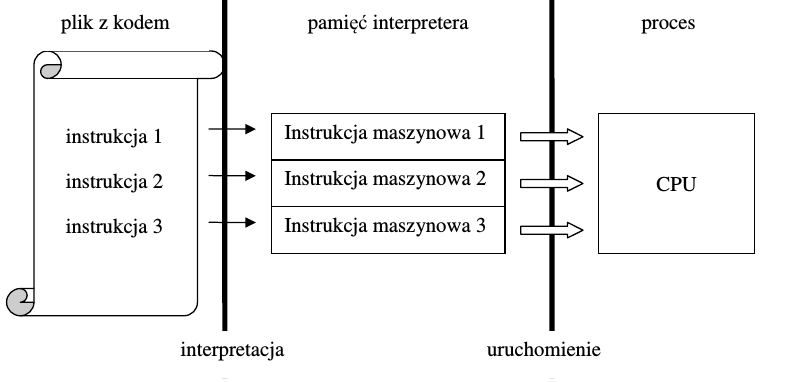
\includegraphics[width=10cm]{diag1}
    \caption{Schemat działania iterpretatora języka skryptowego.}
  \end{figure}
\end{center}
\begin{center}
  \begin{figure}
    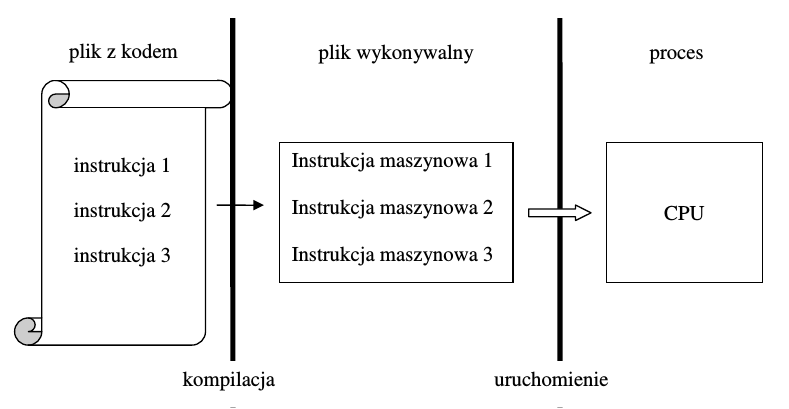
\includegraphics[width=10cm]{diag2}
    \caption{Schemat działania kompilatora.}
  \end{figure}
\end{center}
\subsubsection{Język kompilowalny}
W języku kompilowanym kod programu jest tłumaczony na język maszynowy z pomocą programu
Język kompilowany
zwanego kompilatorem. Program jest przechowywany w postaci kodu maszynowego.
\begin{itemize}
    \tick Wydajne, szybkie i łatwo skalowalne,
    \tick W wielu przypadkach bardziej wydajne od języków skryptowych,
    \tick Często separuje kod od interfejsu, wspierając przejrzystość kodu,
    \tick Za wykrywanie większości błędów odpowiedzialny jest kompilator, który wykrywa
    większość błędów,
    \fail Napisanie aplikacji wymaga więcej pracy niż z językami skryptowymi,
    \fail Bardzo ścisła składnia, wymaga dokładnego programowania,
    \fail Przed uruchomieniem wymagana jest kompilacja, co w dużych projektach wydłuża czas
    znalezienia błędu.
\end{itemize}

\subsubsection{Podsumowanie}
Należy tutaj wspomnieć, że opisane dwie grupy języków nie wskazują, że języki z jednej
grupy są lepsze od języków z drugiej grupy, i języki z jednej grupy należy używać, a
języków z drugiej grupy należy unikać.

\begin{center}
  \begin{tabular}{ll}
    \toprule
    Skryptowe & Ko \\
    \midrule
    Czas & 3 minuty \\
    Cel & Instalacja środowiska pracy potrzebnego podczas całego kursu. \\
    \bottomrule
  \end{tabular}
\end{center}


\subsection{Instalacja środowiska pracy}

\textbf{Uwaga:} Materiał zawarty w tej sekcji jest opcjonalny i jest skierowany głównie do użytkowników systemu
Windows i OS X.
\begin{center}
  \begin{tabular}{lr}
    \toprule
    Forma & Screen cast \\
    \midrule
    Czas & 5 minuty \\
    Cel & Instalacja środowiska pracy potrzebnego podczas całego kursu. \\
    \bottomrule
  \end{tabular}
\end{center}

\subsubsection{Scenariusz}

\begin{itemize}
  \item \emph{W tej części kursu przedstawimy Ci, w jaki sposób zainstalować Pythona i
      całe środowisko pracy.}
  \item \emph{Instalacja środowiska pracy jest bardzo prosta. Istnieją już gotowe pakiety,
    które zawierają interpreter języka Python oraz zestaw bibliotek, z których będziemy
    korzystać podczas trwania kursu.}
\item \emph{Jednym z takich programów jest Anaconda. Wchodzimy na stronę
    \url{www.continuum.io} i przechodzimy do podstrony ''Downloads''. Na stronie możemy
    znaleźć instrukcję instalacji do wszystkich systemów operacyjnych. My skupimy się
    na systemie Windows, ponieważ jest on najmniej dostosowany do języków skryptowych.}
\item \emph{Przechodzimy do sekcji ''Anaconda for Windows'' i wybieramy wersję
    "Python-3.5".}
  \item Program zaczyna się ściągać, trwa to od 1 do 5 minut.
  \item \emph{Program ''Anaconda'' już jest na dysku, możemy przejść do jego instalacji.}
  \item Pokazujemy, że należy klikać ''next''. Sama instalacja trwa również do 5 minut.
  \item \emph{Świetnie. Anaconda została zainstalowana. Możemy sprawdzić, czy wszystko działa,
    wybierając z ''Start'' $\rightarrow$ ''Anaconda'' $\rightarrow$ ''Jupyter
    Notebook''.}
  \item Uruchamiamy program. Po chwili otwiera się przeglądarka internetowa.
  \item \emph{Wszystko działa jak powinno. Możemy zacząć pracę z Pythonem.}
\end{itemize}

\begin{center}
  \begin{figure}
  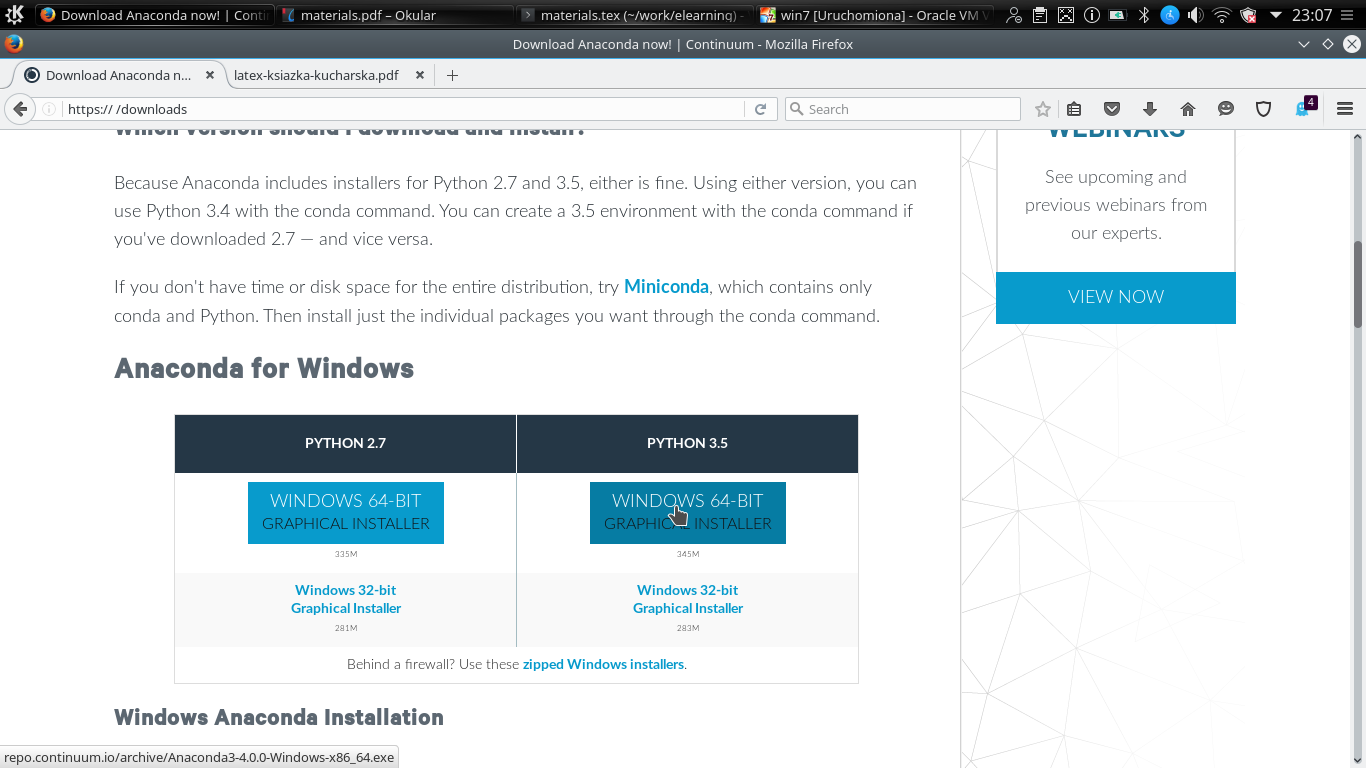
\includegraphics[width=10cm]{install_begin}
  \caption{Strona Anacondy. Kursor wskazuje odpowiedni plik do ściągnięcia.}
  \end{figure}
  \begin{figure}
    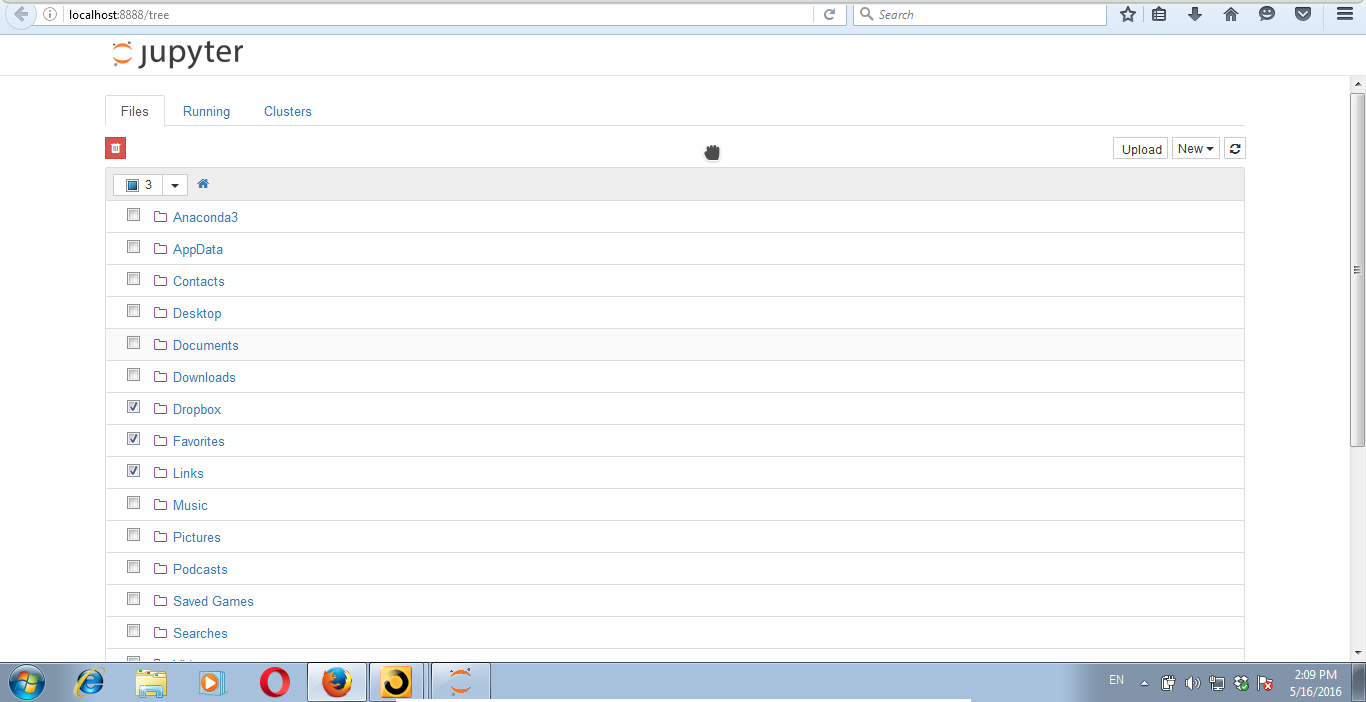
\includegraphics[width=12cm]{install_final}
    \caption{Działający w firefoksie Jupyter Notebook.}
  \end{figure}
\end{center}

\subsection{Pierwsze uruchomienie środowiska}
\begin{center}
  \begin{tabular}{lr}
    \toprule
    Forma & Screen cast \\
    \midrule
    Czas & 3 minuty \\
    Cel & Zapoznanie uczestnika z środowiskiem pracy. \\
    \bottomrule
  \end{tabular}
\end{center}

\subsubsection{Scenariusz}
Końcowy notebook znajduje się w repozytorium: \texttt{notebooks/introToNotebook.ipynb}
\begin{itemize}
  \item \emph{Pokażemy Ci teraz, w jaki sposób korzysta się z IPythona.}
  \item Uruchamiamy \texttt{Ipython Notebook}. Po chwili otwiera sie przeglądarka wraz z
    stroną.
  \item \emph{Stwórzmy nowy notebook.}
  \item Tworzymy nowy notebook i ustawiamy jego nazwę na "Wprowadzenie do IPython
    Notebook".
  \item \emph{Podstawowym elementem notebooka jest komórka, do której
      wpisujemy kod naszego programu. Wpiszmy nasz pierwszy kod do komórki:
    \texttt{print("Hello World!")} i wciśnijmy kombinację "Shift + Enter".}
  \item Wykonał się kod znajdujący się w komórce.
  \item \emph{Widzimy efekt kodu, który był w komórce -- wyświetlił się napis. Pod spodem, została utworzona nowa,
      pusta komórka. Tutaj ponownie możemy wpisać kod, który zostanie przetworzony.}
  \item \emph{Mamy 2 typy komórek, który wybieramy poprzez wybranie z listy znajdującej się w
      \texttt{Cell/Cell Type}. Dwa typy kómórek to \textbf{Code} oraz \textbf{Markdown}. W
    zależności od typu komórki, kod znajdujący się w komórce zostanie inaczej
    zintepretowany.}
\item \emph{Zmieńmy typ komórki na \texttt{Markdown}. Bardzo często chcemy dopisać
    komentarz, który zawiera tekst matematyczny. Z Ipythonem, to nic trudnego: dzięki
    \textbf{MathJaksowi} mamy dostęp do Latexa!}
\item \emph{Należy pamiętać, że samo wpisanie kodu do komórki nic nie zmienia! Za każdym
    razem musimy uruchomić komórkę.}

\end{itemize}

\subsubsection{Zadania}
\begin{enumerate}
  \item Ściągnij z repozytorium notebook \texttt{svd.ipynb}. Notebook zawiera zadania z
    rozkładu macierzy SVD. Jeżeli nie wiesz, co to jest, to nie przejmuj się
    -- nie jest to wcale istotne.
  \item Uruchom kod znajdujący się w komórkach.
  \item Spróbuj wykonać kod w komórkach dwoma skrótami: \texttt{Ctrl + Enter} i
    \texttt{Shift + Enter}. Czy widzisz różnicę w zachowaniu?
  \item Zamień kolejnością dwie ostatnie komórki.
  \item Dodaj jako drugą komórkę, nową komórkę typu \emph{Markdown} i wstaw tekst:
    Niech dana będzie macierz A.
  \item Dodaj do nowostworzonej komórki kod Latexa, który wyświetli macierz A.
  \item Z menu \texttt{Cell} wybierz opcję wyczyszczenia wszystkich wyjść. Czy możemy
    teraz w dowolnej kolejności wywoływać komórki?
\end{enumerate}

\begin{center}
  \begin{figure}
    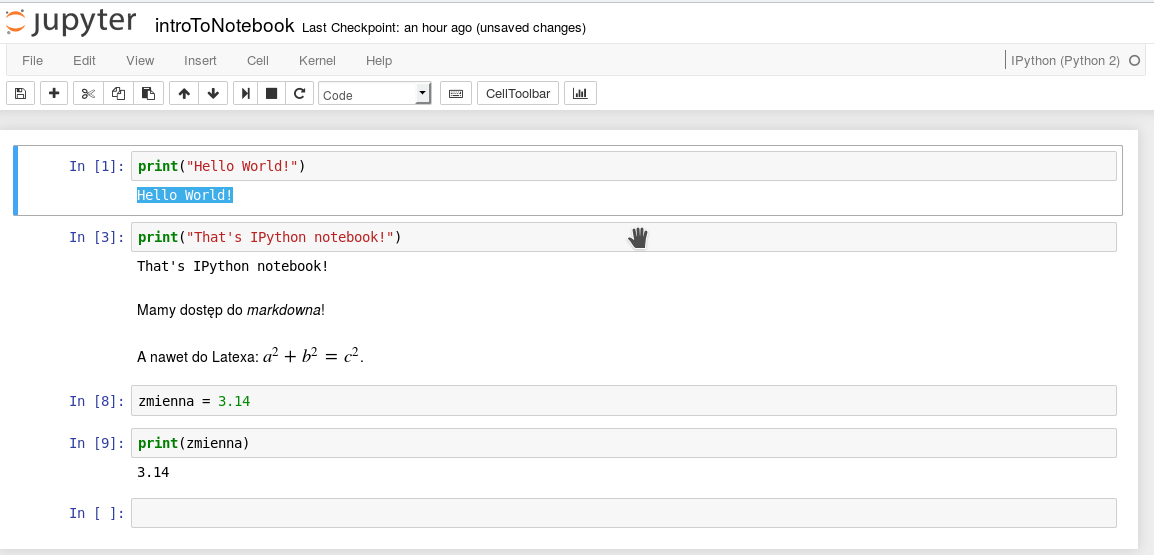
\includegraphics[width=10cm]{zad1}
    \caption{Zadanie 1.}
  \end{figure}
\end{center}

\section{Podstawowe komendy}

\begin{center}
  \begin{tabular}{lr}
    \toprule
    Forma & Screen cast \\
    \midrule
    Czas & 5 minuty \\
    Cel & Zapoznanie uczestnika z podstawowymi elementami Pythona. \\
    \bottomrule
  \end{tabular}
\end{center}
\subsection{Scenariusz}
Końcowy notebook znajduje się w repozytorium: \texttt{notebooks/zmienne.ipynb}
\begin{itemize}
  \item Slajd 1.
  \item \emph{Cześć. W końcu możemy zacząć naukę Pythona. Zobaczysz, że na prawdę jest
      to bardzo prosty język programownia.}
  \item Slajd 2.
  \item \emph{Zaczniemy od bardzo prostego przykładu, który ma na celu wyświetlenie
      napisu na ekran.}
  \item Klikamy na komórkę i wykonujemy kod.
  \item \emph{Widzimy, że pojawił się napis "Hello Python!". Jak pewnie domyślasz się,
      funkcja print jest odpowiedzialna za wypisywanie na ekran. Zgadza się. Dodatkowo,
      podobnie jak w innyh językach, łańcuchy znaków umieszczamy w cudzysłowach.}
  \item Slajd 3.
  \item \emph{Możliwości funkcji print nie ograniczają się do wypisywania łańcuchów
      znakowych. Funkcja print wyświetli nam dowolny typ danych. Popatrzmy, w tej
      komórce przygotowałem kilka przykładów. }
  \item \emph{Tutaj również wyświetlamy łańcuch znaków, ale jest on umieszczony w
      pojedyńczych cudzysłowach. Dla Pythona nie ma to żadnej różnicy.}
  \item \emph{Funkcja print umie wyświetlacz liczby całkowite, jak i zmiennoprzecinkowe.}
  \item \emph{Muszę wspomnieć o jednej przydatnej rzeczy, która jest w Pythonie: możemy
      mnożyć i operować na naprawdę dużych liczbach, nie martwiąc się o przekroczenie
      zakesu.}
  \item \emph{Mamy do dyspozycji wszystkie elementarne operacje arytmetyczne: od
      dodawania do potęgowia. Właśnie taki zapis -- dwie gwiazdki -- oznacza
      potęgowanie. Możemy dodatkowo umieszczać nawasy.}
  \item \emph{Bardzo często się zdarza, że chcemy wydrukować kilka rzeczy naraz, np.
      opis zmiennej i jej zawartość. Nic trudnego, poszczególne elementy oddzielamy
      przecinkiem. Python oddzieli je spacja dla zwiększena czytelności.}

  \item Slajd 3.
  \item \emph{Następną przydatną rzeczą, którą pewnie znasz z innych języków
      programowania, są komentarze. Komentarz, czy fragment kodu, który zostanie
      pominięty podczas interpretownia kodu. W Pythonie, komentarza zaczynają się od
      znaku hasha. Wszystko, co znajduje się za nim, zostanie pominięte.}
  \item Slajd 4.
  \item \emph{Zobaczmy następujący przykład. Mamy fragment kodu, który wyświetli nam
      napis "Ala ma kota.". Tuż za nim rozpoczyna się komentarz. Drugi wiersz jest
      całkowicie zakomentowany, więc interpretor powinien go pominąć.}
  \item Uruchamiamy kod z komórki.
  \item \emph{Widzimy, że wykonał się kod, który znajduje się w pierwszej linii. Zgodnie z
      naszymi przewidywaniami.}
  \item Slajd 5.
  \item \emph{Podstawowymi elementami języków programowania są zmienne. Służą one do
      przechowywania np. obliczeń. W Pythonie nazwy zmiennych są czułę na wielkość
      liter: zmienna zmenna pisana małymi literami jest różna od tej pisanej wielkimi.}
  \item \emph{Kiedy tworzomy zmienną w Pythonie, to nie musimy podawać jej typu. Zmienna
      zawsze ma tym obiektu, którzy przechowuje! Nie ma też problemu, żeby zmienna
      zmieniła swój typ podczas trwania programu, wystarczy przypisać nową wartość.}
  \item Slajd 6.
  \item \emph{Podobnie jak w innych językach programowania, przypisanie następuje przy
      pomocy znaku równości. Pierwszy przykład pokazuje, że zmienna może zmienić typ
      podczas trwania programu. Mamy 4 podstawowe typu: całkowito-liczbowy,
      zmienno-przecinkowy, łąńcuchy znaków i typ logiczny.}
  \item Slaj 7.
  \item \emph{Funkcja type zwraca nam typ obiektu, który możemy wyświetlić. Widzimy, że
      np. zmienna ocena\_z\_pythona jest typu całkowito-liczbowego.}
  \item \emph{W tej części kursu poznałeś w jaki sposób wyświetlić w Pythonie różnego
      rodzaju wyrażenia, w jaki sposób pisze się komentarze oraz jak korzystać z
      zmiennych. Zapraszam teraz do rozwiązania kilku zadań, króre pozwolą Ci utrwalić
      materiał zawarty w tej cześci kursu.}
\end{itemize}

\subsection{Zadania}
Zadania do tej części znajduje się w repozytorium: \texttt{notebooks/zmienne\_zadania.ipynb}

\section{Listy jako odpowiednik tablic}
\begin{center}
  \begin{tabular}{lr}
    \toprule
    Forma & Screen cast \\
    \midrule
    Czas & 15 minuty \\
    Cel & Zapoznanie uczestnika z listami. \\
    \bottomrule
  \end{tabular}
\end{center}
\subsection{Scenariusz}
Notebook wykrzystywany podczas prezentacji znajduje się w repozytorium: \texttt{notebooks/listy.ipynb}
\begin{itemize}
  \item Slajd 1.
  \item \emph{Cześć. W tej cześci kursu powiemy Ci, w jaki sposób możesz wykorzystać
      listy z Pythona. }
  \item Slajd 2.
  \item \emph{W Pythonie nie istnieją tablice znane Ci z innych języków
      programowania. Python posiada listy, które bardziej przypominają strukturę danych
      zwaną wektorem w C++ lub Javie. Listy pozwalają zrobić o wiele więcej rzeczy. Jak
      wcześniej zauważyliśmy, Python nie zwraca za bardzo uwagi na typ zmiennych.
      Podobnie jest z listami: w jednej liście możesz posiadać elemenety różnych typów. }
  \item \emph{Tak jak w innych językach, indeksowanie zaczyna się od 0. Zobaczmy kilka
      przykładów.}
  \item Slajd 3.
  \item \emph{utworzenie listy jest bardzo proste: orbimy to przez nawiasy kwadratowe
      (z angielskiego brackety). Podczas tworzenia listy możemy od razu wpisać do niej
      kilka elementów.}
  \item \emph{Jak wcześniej powedziałem, w listach możemy przechowywać obiekty różnych
      typów. Zobaczmy, lista roznosci składa sie z liczby zmiennoprzecinkowej, łańcucha
      znakowego, listy, jak i liczby całkowitoliczbowej.}
  \item \emph{Python posiada wbudowe funkcje, które tworzą nam listy o konkretnych
      elementach. Najpopularniejszą taką funkcją jest range, która zwraca
      n elementową listę, zaczynając od zera. Jak tutaj, range(10) zwróci nam
      listę elementów od zera do dziewięciu.}
  \item Slajd 4.
  \item \emph{Pythonowe listy mogą być zmieniane podczas trwania skryptu: możemy dodać ,
      jak i odejmować elementy. Jeżeli chcemy dodać nowy element do listy, to możemy
      skorzystać z metody append(), która dodaje element przekazany jako argument na
      koniec listy. W tym przypadku dodamy liczbę 6 na koeniec listy oceny. Innym
      sposobem na dodanie elementów do listy jest rozszerzenie jej o inną listę. Do tego
      służy metoda extend. Jak się domyślasz, metod pop jest odpowiedzialna za usuwanie
      elementów z listy.}
  \item Slajd 5.
  \item \emph{Python posiada rozbudowany sposób indeksowania, tj. pobierani konkretnego
      elementu z listy. Jeżeli chcemy pobrć pierwszy element z listy, pobieramy go przy
      pomocy indeksu zero. }
  \item \emph{Ale Python posiada również indeksowanie ujemne, które pozwala na
      pobieranie elementów od końca. Jeżeli chcemy pobrać ostatni element z listy,
      możemy wykorzystać indeks -1, przedostatni -2.}
  \item \emph{Indeksowanie nie ogranicza się tylko po pobierania pojedyńczych elementów.
      Możemy użyć drukropka, żebu uzyskać konkretną podlistę. Tak jak tu: zapis ":5"
      zwróci mam 5 pierwszych elementów, a "-5:", pięć ostatnich. Mówiąc ogólnie, zapis
      "A:B" zwróci nam podlistę zaczynającą się od indkesu A, aż do indeksu B.}
  \item \emph{Jeżeli dodamy jeszcze jeden dwukropek, to powiemy, co który element
      chcemy. Na przykład zapis "::2" zwróci nam co drugi elementem, a "::-1" zwróci nam
      odwróconą listę.}
  \item Slajd 6.
  \item \emph{Listy w Pythonie pozwalają na kilka przydatnych operacji. Podstawowym operacją
      jest operacja sortowania -- służy do tego metoda sort(). Możemy odwrócić listę
      dzięki metodzie reverse() albo zliczyć ile razy dany element wystąpił w liście.}
  \item Slajd 7.
  \item \emph{Python posiada odmienną do innych języków pętle for. Pętla for
      wykorzystuje listy i iteruje po nich, tak samo jak pętle foreach z innych
      języków. A w jaki sposób napisać pętle, która ma mieć konkretną liczbę iteracji?}
  \item Slajd 8.
  \item \emph{Nic trudnego. Pamiętasz funkcję range? Zwraca ona listę o konkretnej
      liczbie elementów. Widzimy, że zmienna i przechodzi po calej liście. Do pętli
      mozemy przekazać dowolną listę, np. listę oceny, którą wcześniej stworzyliśmy.}
  \item Slajd 9.
  \item \emph{Powiedzmy, że potrzebujemy listę zawierającą kwadraty liczb od 0 do 9. W
      Pythonie, to nic trudnego. Tworzymy pustą listę. Następnie w pętli, która wykona
      się 10 razy, dodajemy następne kwadraty. }
  \item \emph{Dotarliśmy do końca tej części kursu. Możesz być przestraszony liczbą
      materiału, ale uwierz mi, że odrobina praktyki pozwoli zrozumieć, że listy są
      przyjemne w korzystaniu i proste.}
\end{itemize}

\section{Funkcje w Pythonie}
\begin{center}
  \begin{tabular}{lr}
    \toprule
    Forma & Screen cast \\
    \midrule
    Czas & 5 minuty \\
    Cel & Zapoznanie uczestnika z funkcjami. \\
    \bottomrule
  \end{tabular}
\end{center}

\subsection{Scenariusz}
Notebook wykrzystywany podczas prezentacji znajduje się w repozytorium:
\texttt{elearning/funkcje.ipynb}
\begin{itemize}
  \item Slajd 1.
  \item \emph{Zanim przejdziemy do zadań, to potrzebujesz jeszcze dowiedzieć się w jaki
      sposób działąją funkcje w Pythonie i jak napisać własne.}
  \item Slajd 2.
  \item \emph{Do zdefiniowania własne funkji służy słowo kluczowe <def>, po której
      następuje nazwa funkcji, a w nawiasach podajemy listę argumentów. Podobnie jak w
      C++ lub Javie, z tą różnicą, że nie interesują nas typy argumentów oraz typ, jaki
      zwraca funkcja.}
  \item \emph{Zobaczmy przykład. Mamy tu funkcję, która zwraca True, jeżeli element jest
      większy od pięciu, zaś w przeciwnym przypadku zwróci False. Funkcja nazywa się
      is\_greater\_than\_5 i przyjmuje jeden argument --  x. Do zwrócenia wartości z
      funkcji, służy słowo kluczone <return>. Tak samo, jak w innych językach
      programowania. Możemy teraz przejść do zadań.}
\end{itemize}

\section{Zadanie z list i funkcji}
\begin{center}
  \begin{tabular}{lr}
    \toprule
    Forma & Screen cast i praca z notebookiem \\
    \midrule
    Czas & 30 minuty \\
    Cel & Utwralenie wiedzy z poprzednich części. \\
    \bottomrule
  \end{tabular}
\end{center}
Notebook wykrzystywany podczas prezentacji znajduje się w repozytorium:
\texttt{tasks/zadania\_1.ipynb}
\subsection{Scenariusz}
\begin{itemize}
  \item Otworzony notebook z zadaniami.
  \item \emph{Cześć. W tej części zajęć będzisz musiał napisać swój własny kod w
      Pythonie. Wszytkie zadania polegają na napisaniu konkretnej funkcji, które
      muszą zwrócić konkretny wynik.}
  \item \emph{Każde zadanie składa się z trzech elementów: treści, komórki, gdzie
      powinienieś umieścić swój kod oraz kilku testów, które mają potwierdzić, że dobrze
      napisałeś kod.}
  \item \emph{Zanim jeszcze zaczniesz pisać kod, zobacz notebook, z filmiku i przypomnij
      sobie wszystkie poznane elementy. Na pewno będziesz musiał z nich skorzystać.
      Jeżeli będziesz miał problemy z rozwiązaniem konkretnego zadania -- nie przejmuj
      się -- i spróbuj znaleźć podpowiedź w internecie. Na pewno ktoś miał podobny
      problem do Twojego. Powodzenia!}
\end{itemize}

\end{document}
